\section{Systèmes d'administrations}\label{sec:rw:supervision:administration}
Depuis le début des années 80, grâce aux premières mises en réseau d'équipements, les systèmes d'administrations permettent de gérer des parcs de ressources. Le principe est de surveiller et surtout contrôler un système afin qu'il satisfasse les demandes des utilisateurs et les contraintes du propriétaire~\cite{Sloman:management}. Dans cette thèse, nous nous intéressons à l'observation, le contrôle (par rétroaction par exemple) est en dehors du périmètre de cette étude. Pour permettre la surveillance, chaque objet d'un système va représenter son état dans un modèle qui est consultable via un protocole.

Cette section présente les systèmes d'administrations déployés pour exploiter des parcs de dispositifs à grande échelle. Ces systèmes sont spécifiés au travers de divers consortiums ou forums. Les principaux acteurs sont : le \textit{BroadBand Forum} (BBF) (porté par les opérateurs télécoms du monde de l'accès internet résidentiel), le \textit{Forum Universal Plug'n'Play} (UPnP) (porté par l'électronique grand publique), ou encore \textit{Distributed Management Task Force} (DMTF), l'\textit{Institute of Electrical and Electronics Engineers} (IEEE) et l'\textit{Internet Engineering Task Force} (IETF), organisations ouvertes où participent entreprises, laboratoires et indépendants. Ces ententes permettent la spécification des standards autant au niveau des protocoles de communications que sur la structure des données manipulées en terme de modèle ou de schéma.

Cette section présente d'abord la structure et la gestion des données issues des ressources administrées. Ensuite, nous analysons l'ensemble des possibilités de traitement fournies par ce type de systèmes. Et enfin, une synthèse est présentée grâce à notre grille d'analyse.
\subsection{Gestion des données pour l'administration}
L'architecture de la gestion des données dans les systèmes classiques d'administration est principalement fondée sur des gestionnaires \enquote{agents}~\cite{CCITT:X700} (voir fig.~\ref{fig:rw:supervision:administration}). Cette architecture est celle utilisée de nos jours dans les protocoles d'administrations tels que TR-069~\cite{BBF:tr069}, UPnP Device Management~\cite{UPnP:DM2}, mais aussi sur des protocoles plus anciens tels que SNMP~\cite{IETF:SNMP}. Le principe est qu'un module logiciel est présent sur les dispositifs devant être administrés. Celui-ci comporte un agent capable de maintenir une petite \enquote{base de données} sous une forme particulière représentant les données et états du système. Un gestionnaire est capable par la suite de transmettre les informations de l'agent à un système d'administration global. Ce dernier agrège ainsi l'ensemble des dispositifs.
\begin{figure}[ht]
    \centering
    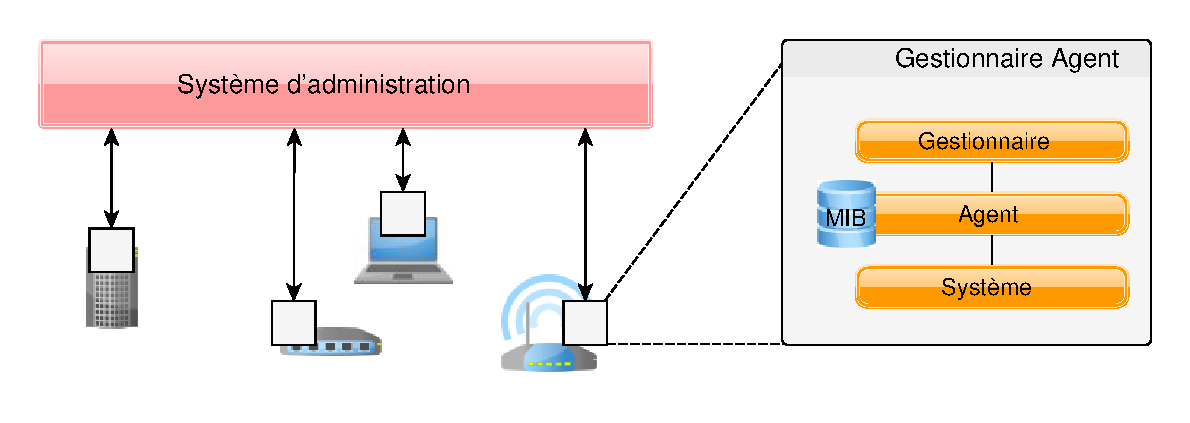
\includegraphics[width=.70\textwidth]{fig/rw-supervision-administration}
    \caption{Agent d'administration sur un dispositif}\label{fig:rw:supervision:administration}
\end{figure}

\subsubsection{Les données fournies par les agents}
Il existe plusieurs structures de données dans le cadre des systèmes d'administrations. La structure la plus répandue reste la \textbf{structure hiérarchique}. La première apparition d'un tel modèle dans ce domaine remonte à la spécification de SNMP~\cite{IETF:SNMP} qui décrit le concept de \textit{Management Information Base} (MIB)~\cite{IETF:MIB}. Une \textit{MIB} est une base d'information où les données sont regroupées sous forme d'arbre. Chaque information possède un chemin unique (l'\textit{object identifier}) décrit par une suite de chiffres séparés de points. Des catalogues répertorient l'ensemble des \textit{MIB} existantes (standardisées ou non)\footnote{\url{www.mibsearch.com} ou \url{www.mibdepot.com} par exemple}.

Les protocoles récents permettent aussi de manipuler des données de manière hiérarchique sur les agents. Le protocole TR-069 spécifie l'accès distant à un modèle de données décrit dans le document technique \textit{TR-106}~\cite{BBF:tr106}. Le protocole UPnP-DM permet aussi l'accès à un modèle par le réseau local via le service de gestion de configuration (CMS)~\cite{UPnP:DMCMS}. Dans ces derniers, les structures de données sont toutes les deux hiérarchiques.

Un exemple de ce type de structure est présenté en figure~\ref{fig:rw:supervision:dmtree}. Une donnée est définie de manière unique, tout comme dans une \textit{MIB}, grâce à son chemin complet. Dans le vocabulaire du domaine de l'administration, cette donnée est appelée \textit{paramètre}. Le \textit{chemin} d'un paramètre est la concaténation des noms des nœuds qui le sépare de la racine, avec pour séparateur \enquote{/} dans UPnP ou \enquote{.} dans TR-069. L'implémentation de l'agent permet de créer et de remplir cette base d'information.

\begin{figure}[ht]
    \centering
    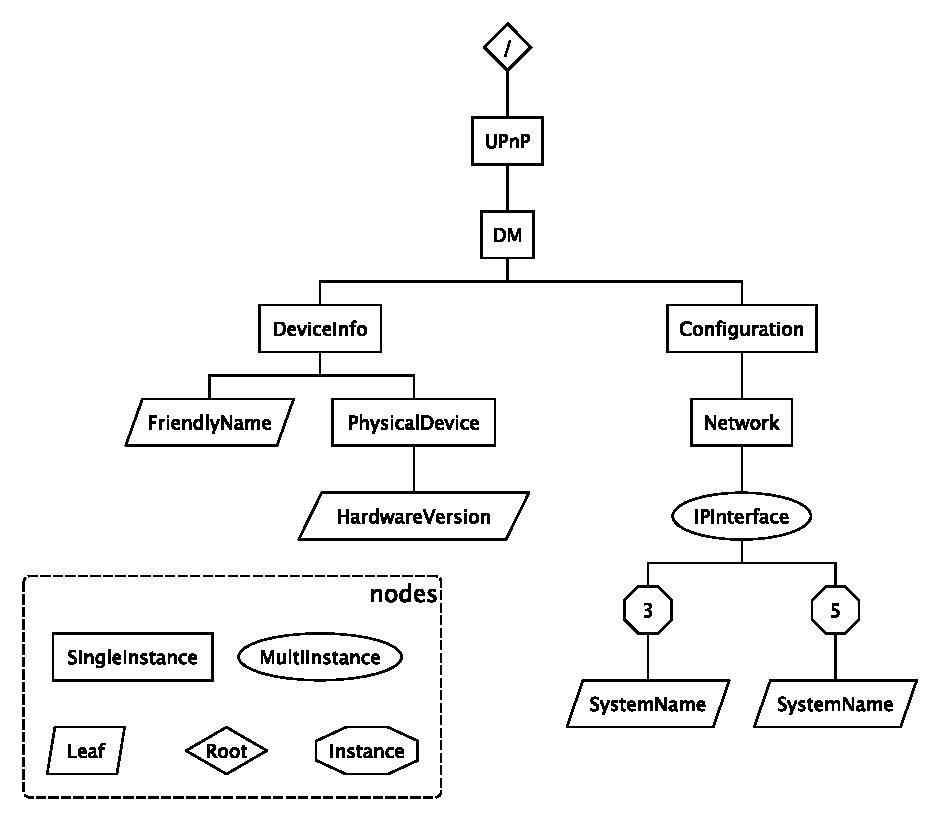
\includegraphics[width=.5\textwidth]{fig/rw-supervision-dmtree}
    \caption{Structure hiérarchique du modèle de données d'UPnP-DM}\label{fig:rw:supervision:dmtree}
\end{figure}

Toutefois, tous les modèles ne sont pas structurés sous forme de hiérarchie. Par exemple, la DMTF a adopté le modèle objet. En effet, dans les protocoles tels que WS-MAN~\cite{DMTF:WS-MAN}, le schéma conceptuel \textit{CIM} (\textit{Common Information Model})~\cite{DMTF:CIM} est décrit par un diagramme de classe UML comme présenté en figure~\ref{fig:rw:supervision:cimcore}. Ces protocoles sont notamment utilisés pour l'administration de web-services et applications entreprises. 

\begin{figure}[ht]
    \centering
    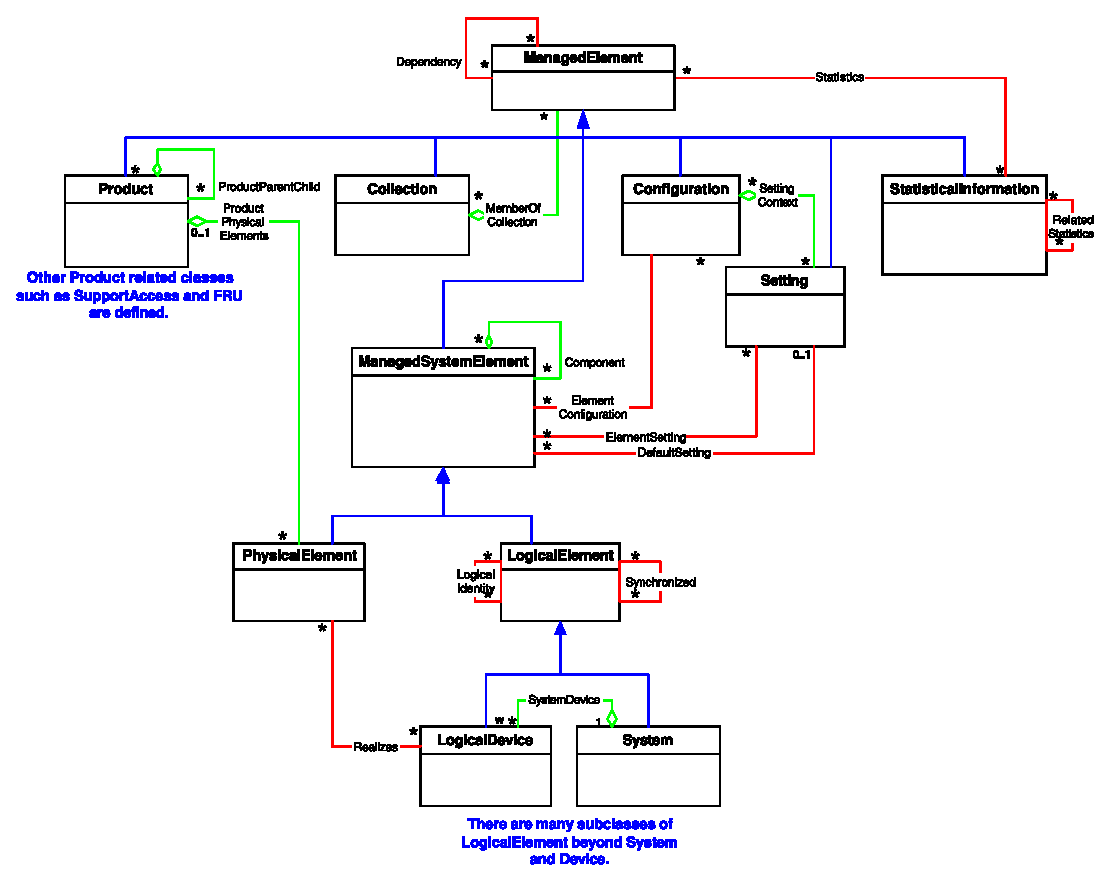
\includegraphics[width=.50\textwidth]{rw-supervision-cimcore}
    \caption{Modèle de classe de la partie \textit{Core} de \textit{CIM}}\label{fig:rw:supervision:cimcore}
\end{figure}

Plusieurs extensions standardisées existent pour représenter les différents types d'objets faisant partie des systèmes observés : Base de données, Dispositifs, Réseau, Sécurité, Utilisateur, Applications\dots{} Ainsi, le modèle de données est un modèle d'objet respectant l'ensemble des spécifications et des extensions. L'inconvénient majeur d'un tel choix reste la complexité de \textit{CIM} qui se trouve souvent réduite pour être applicable en pratique~\cite{Lopez:datacenter}.

Pour accéder aux données, le système se compose de multiples agents qui sont une représentation de chaque objet. Nous pouvons noter que ce principe reste le même pour l'administration de modules Java dans le protocole JMX~\cite{Sun:JMX} où des objets particuliers (les \textit{MBean}) sont exposés et peuvent être consultés et manipulés via ce protocole.

\subsubsection{Gestion de l'évolution des données}
Pour les différentes solutions présentées, les agents ont toujours trois modes principaux pour fournir des données :
\begin{itemize}
	\item[\textbf{Consultation indirecte}: ] Ce fonctionnement est le plus simple. La donnée est stockée dans une base d'information. Au moment de la consultation, l'agent lit directement dans la base et renvoie l'information.
	\item[\textbf{Consultation active}: ] Au moment de la consultation de la donnée via une primitive comme \enquote{\it get}, l'agent va effectuer le relevé actif de la donnée à la source. Ce relevé peut potentiellement prendre plus de temps qu'une simple lecture dans une base d'information.
	\item[\textbf{Événement}: ] La plupart des systèmes d'administrations supportent un mécanisme de \textit{publish}/\textit{subscribe} permettant de créer des canaux d'événements. La création d'événement se fait à partir du changement de valeur d'un paramètre ou à la création d'objets (ou de chemins).
\end{itemize}

Toutefois, la consultation et les canaux d'événements sont deux approches et deux mécanismes différents qui sont rarement intégrés.

\subsubsection{Le gestionnaire global}
Le système d'administration est capable de se connecter à une multitude d'agents. Ainsi, il peut constituer la vue globale du système par l'intégration des données.

Il est important de noter que ce système peut être réparti pour mieux amortir la charge en la présence de grandes quantités d'agents à administrer. Toutefois, pour l'administration de ses dispositifs, \textit{France Telecom} utilise un point central d'administration : l'\textit{ACS} (\textit{Auto-configuration Server}, serveur d'administration en TR-069). En effet, la fréquence d'émission des données en fonctionnement normal est lente (pour chaque dispositif, un rapport par jour typiquement). Pour les 10 millions d'équipements à gérer, une capacité de 500 réceptions par seconde côté serveur est suffisante. Cette capacité est atteinte sur des \textit{ACS} récents tels que \textit{EDGE}~\cite{Motorola:EDGE} de \textit{Motorola} sur des serveurs de puissance moyenne.

Pour permettre de supporter la charge des informations remontées, plusieurs systèmes d'administrations proposent des architectures décentralisées (principalement hiérarchiques) pour la gestion à plus grande échelle~\cite{Kessis:management}. La hiérarchie peut se découper par lieu géographique, ou par domaine d'activité.

Nous venons de voir comment les systèmes d'administrations sont structurés et notamment comment ces systèmes modélisent leurs données. La section suivante présente les capacités de traitements de ce type de systèmes.

\subsection{Possibles traitements de données}
Que ce soit au niveau de l'agent comme au niveau du gestionnaire global, les données peuvent être traitées. Cette section détaille les différentes possibilités. Tout d'abord, nous voyons comment l'hétérogénéité des systèmes est traitée et comment l'intégration des multiples agents se fait. Par la suite, nous détaillons l'ajout de nœuds particuliers comme calcul de statistiques ou l'ajout de fonctions tierces.

\subsubsection{L'hétérogénéité par l'uniformisation des modèles}
La standardisation est un enjeu majeur pour les systèmes d'administrations à grande échelle. Comme présentés précédemment, la spécification les protocoles d'administrations se fait au sein de consortiums. Ainsi, la gestion de l'hétérogénéité s'appuie sur le respect des standards. Suivant les dispositifs observés, différents profils existent. Que ce soit pour les profils hiérarchiques ou à objet, des spécifications sont écrites pour décrire le modèle de données.

La gestion de l'hétérogénéité se fait par la description de profils standardisés. L'intégration de protocoles équivalents est un domaine à part entière dans lequel plusieurs approches ont été proposées~\cite{Kaed:these}. Enfin, remarquons que plus le nombre de domaines d'intérêt, plus le nombre de spécifications à considérer augmente.

\subsubsection{Intégration de sources}
L'avantage principal d'utiliser des modèles standards est l'intégration des sources de données. En effet, comme chacune des entités du système répond à un profil prédéfini, il est possible de faire l'union des données par catégorie pour avoir toutes les entités répondants aux différents profils. Ainsi, les données sont naturellement intégrées dans un modèle commun, ce qui permet aux concepteurs de systèmes d'observations de fournir des fonctions très avancées sans pour autant connaître l'instance du système. De plus, plusieurs protocoles et standards peuvent être utilisés dans un même système, comme l'a proposé WBEM~\cite{DMTF:WBEM}, dans lequel des objets SNMP, JMX et autres sont intégrés à un modèle commun CIM.

Une fois les données accessibles à un niveau global, il devient possible de traiter ces données afin de les analyser, ou former des alertes. Pour cela, les systèmes d'administrations ne fournissent pas tous les mêmes capacités. Par défaut, la seule capacité que peut fournir l'agent est la récupération de son modèle de données (ou une sous-partie). Cependant, plusieurs systèmes permettent à l'utilisateur de définir des processus plus complexes pour permettre un traitement de plus haut niveau.

L'approche la plus utilisée est le \textit{scripting}. Le système d'observation fournit à l'utilisateur un langage \textbf{impératif} qui lui permet de définir des routines. Par exemple, EDGE~\cite{Motorola:EDGE} fournit une interface \textit{Javascript}, et l'\textit{ACS} d'\textit{Alcatel-Lucent} permet d'utiliser des programmes \textit{Python}. Ces routines peuvent par la suite être intégrées dans des réponses aux événements, ou dans des procédures de diagnostics ou encore de configuration.

Il est notable que les standards WBEM et WS-MAN définissent un langage \textbf{déclaratif} de manipulation de modèles CIM, le \textit{CQL} (\textit{CIM Query Language})~\cite{DMTF:CIM-QL}. Ce langage est très similaire à \textit{SQL} utilisé dans un cadre relationnel-objet. Dans sa spécification, il permet toutes les fonctionnalités de \textit{SQL} (sélection, projection, jointure, agrégation, imbrication de requêtes). Il est aussi utilisé afin de définir des filtres plus précis sur les événements (en remplacement du langage par défaut \textit{XPath}). Il est intéressant de noter que ce langage permet aussi la définition de \textit{politiques de gestions}, assimilables à des routines événements-condition-action. Toutefois, il reste peu implémenté dans la pratique.

\subsubsection{Sur l'agent : paramètres calculés}
Dans chacune des solutions présentées, il existe des parties du schéma de données consacrées à la présentation de statistiques. En effet, pour un paramètre dont la valeur représente une mesure, il peut être intéressant de fournir des extremums ou moyennes calculées à la volée. Plusieurs standards intègrent un tel calcul principalement sur un échantillon précis ($N$ données) avec un ensemble fixé d'opérateurs.

Tous les modèles présentés sont extensibles à volonté. Par exemple, sous UPnP-DM et TR-069, il est autorisé de rajouter des branches à l'arbre de données sous l'appellation \verb|X_{ORGANISATION}| (par exemple \verb|X_ORANGE_COM|). Ainsi, cela permet aux développeurs de fournir des données non prévues dans les standards ou pour rajouter de fonctionnalités de traitement.

\subsection{Synthèse}
Le tableau~\ref{tab:rw:supervision:administration:synthese} résume l'ensemble de l'analyse menée sur les systèmes d'administrations. L'ensemble permet effectivement beaucoup de fonctionnalité pour les utilisateurs. Le choix de s'appuyer sur des standards fait que cette approche est actuellement très répandue pour gérer des systèmes de tous types. Ce qui en fait un excellent système pour collecter les données sur les ressources du système. Toutefois, l'interrogation des données est majoritairement faite dans un langage non déclaratif. De plus, les canaux événementiels et la consultation des bases d'informations sont gérés dans des approches et mécanismes très différents. Ceci rend une observation intégrée difficile.


\begin{table}[!ht]
\criteretabDonnee
    {Principalement modèle \textbf{hiérarchique} sous forme de système de fichier. Quelques systèmes d'administration utilisent des modèles objets avec \textit{CIM}.}
    {Les différentes entités du système sont des nœuds du modèle. Pas de contraintes ou d'inférences exprimables.}
    {Le dynamisme est géré par le mode d'accès. Certaines données peuvent être notifiables. Les mécanismes d'interrogations sont séparés.}
\criteretabTraitement
    {Instantanée et continue sur certaines données. Pas d'hybride possible vu que les procédés sont très séparés.}
    {Standardisation des modèles. Toutes les entités sont structurées dans le même formalisme. Intégration par union des données pour chaque profil.}
    {Appel de méthodes standards pour récupérer un sous-arbre du modèle. Code impératif (scripting) principalement pour manipuler les données au niveau du gestionnaire. Utilisation de langage déclaratif (similaire SQL ou XPath) possible.}
    {Procédures à écrire en \textit{script}. Projection, sélection et union principalement. Certains nœuds particuliers permettent de calculer des statistiques.}
\criteretabAdaptabilite
    {Pas d'adaptation spécifique, car les dispositifs doivent implémenter des standards.}
    {Pas de perspectives métiers en dehors de la sélection sur les branches du modèle.}
    {Nœuds particuliers pour le calcul. Fonctions métiers intégrées dans le gestionnaire.}
    {Très efficace et utilisé pour gérer des parcs de millions de dispositifs.}
\caption{Synthèse des systèmes d'administration}\label{tab:rw:supervision:administration:synthese}
\end{table}